\documentclass[11pt,a4paper]{article}

% -------------------------------------------------
% PAQUETES BÁSICOS
% -------------------------------------------------
\usepackage[utf8]{inputenc}
\usepackage[T1]{fontenc}
\usepackage[spanish]{babel}
\usepackage{lmodern}
\usepackage{amsmath,amssymb,amsfonts,amsthm}
\usepackage[margin={2.6cm,2.6cm}]{geometry}

% Código fuente
\usepackage{xcolor}
\usepackage{listings}
\usepackage{hyperref}


\usepackage{fontawesome5}
\usepackage{dirtree}

\definecolor{git}{HTML}{F1502F}
\definecolor{azuluc}{HTML}{1F4E79}

\lstdefinestyle{latexstyle}{
    language=[LaTeX]TeX,
    basicstyle=\ttfamily\small,
    keywordstyle=\color{blue!70!black},
    commentstyle=\color{green!40!black},
    stringstyle=\color{red!70!black},
    numberstyle=\tiny\color{gray},
    numbersep=8pt,
    breaklines=true,
    breakatwhitespace=false,
    frame=single,
    rulecolor=\color{gray!50},
    backgroundcolor=\color{gray!5},
    showstringspaces=false,
    morekeywords={newtheorem,DeclareMathOperator},
    tabsize=4,
    literate=
    {á}{{\'a}}1
    {é}{{\'e}}1
    {í}{{\'i}}1
    {ó}{{\'o}}1
    {ú}{{\'u}}1
    {Á}{{\'A}}1
    {É}{{\'E}}1
    {Í}{{\'I}}1
    {Ó}{{\'O}}1
    {Ú}{{\'U}}1
    {ñ}{{\~n}}1
    {Ñ}{{\~N}}1
    {ü}{{\"u}}1
    {Ü}{{\"U}}1
    {¡}{{\textexclamdown}}1
    {`}{\textasciigrave}1
    {´}{\textquotesingle}1,
}

\lstset{style=latexstyle}


% Cajas de contenido
\usepackage[most]{tcolorbox}

\newtcolorbox{paginarecuadrada}[1][]{
    colback=white,
    colframe=black,
    boxrule=0.8pt,
    arc=0mm,
    width=\textwidth,
    left=5mm,
    right=5mm,
    top=5mm,
    bottom=5mm,
    enhanced,
    breakable,
    #1
}




\theoremstyle{plain}
\newtheorem{teorema}{Teorema}
\newtheorem{proposicion}[teorema]{Proposición}
\newtheorem{corolario}[teorema]{Corolario}
\newtheorem{lema}[teorema]{Lema}

\theoremstyle{definition}
\newtheorem{definicion}{Definicion}
\newtheorem{ejemplo}{Ejemplo}

\theoremstyle{remark}
\newtheorem{observacion}{Observacion}


\newtheoremstyle{exercise}{0.8em}{0.8em}{\normalfont}{}{\bfseries\color{azuluc}}{.}{0.5em}{}
\theoremstyle{exercise}
\newtheorem{exercise}{Ejercicio}




\newcommand{\R}{\textcolor{azuluc}{\faIcon{r-project}}}
\newcommand{\Git}{\textcolor{git}{\faIcon{git-alt}}~\!Git}
\newcommand{\GitHub}{\faIcon{github}~\!GitHub}
\newcommand{\Markdown}{Markdown~\faIcon{markdown}}
\newcommand{\checkicon}{\textcolor{verde}{\faIcon{check}}}
\newcommand{\crossicon}{\textcolor{rojo}{\faIcon{times}}}



% -------------------------------------------------
% DATOS DEL DOCUMENTO
% -------------------------------------------------

\title{\LARGE\textbf{Práctica 11: Entornos en \LaTeX}\\[0.5em]
\Large Laboratorio de Matemáticas\\
\small\ \\
\Large Grado en Ingeniería Matemática - Doble Grado en Física e Ingeniería Matemática}
\author{Miguel Beltrá Vidal}
\date{Curso 2026/27}


% -------------------------------------------------
% DOCUMENTO
% -------------------------------------------------
\begin{document}

\maketitle

\section{Objetivos}

El objetivo de esta práctica es continuar aprendiendo los fundamentos de \LaTeX, prestando especial atención a la organización del texto, la creación de listas, tablas, matrices, ecuaciones alineadas y entornos matemáticos. Al finalizar, el estudiante deberá ser capaz de:
\begin{itemize}
    \item Alinear texto de diferentes formas mediante los entornos \verb|center|, \verb|flushleft| y \verb|flushright|.
    \item Crear listas numeradas y no numeradas.
    \item Construir tablas, matrices y estructuras tabulares en modo matemático.
    \item Alinear expresiones matemáticas mediante el entorno \verb|align|.
    \item Utilizar entornos matemáticos predefinidos y crear
    sus propios entornos de tipo teorema, definición o lema.
\end{itemize}

% =================================================
% 1. ALINEACIÓN DE TEXTO
% =================================================

\section{Alineación de texto}

\LaTeX\ permite modificar la alineación del texto mediante diferentes entornos. Los tres más habituales son \verb|center|, \verb|flushleft| y \verb|flushright|.

\subsection{Entorno \texttt{center}}

El entorno \verb|center| permite centrar horizontalmente el texto o los elementos que contiene.

\begin{lstlisting}
Texto normal alineado a la izquierda.

\begin{center}
    Texto centrado.
\end{center}
\end{lstlisting}

\noindent El resultado será:

\begin{paginarecuadrada}
Texto normal alineado a la izquierda.

\begin{center}
    Texto centrado.
\end{center}
\end{paginarecuadrada}

%Este entorno puede utilizarse tanto para texto como para otros elementos, por ejemplo, tablas, imágenes o expresiones matemáticas.
%
%\medskip
%
%\begin{lstlisting}
%\begin{center}
%    \[
%        x^2+y^2=z^2
%    \]
%\end{center}
%\end{lstlisting}
%
%\noindent El resultado será:
%
%\begin{paginarecuadrada}
%\[
%    x^2+y^2=z^2
%\]
%\end{paginarecuadrada}

\subsection{Entorno \texttt{flushleft}}

El entorno \verb|flushleft| permite alinear el contenido a la izquierda.

\begin{lstlisting}
\begin{flushleft}
    Este texto aparece alineado a la izquierda.
\end{flushleft}
\end{lstlisting}

\noindent El resultado será:

\begin{paginarecuadrada}
\begin{flushleft}
    Este texto aparece alineado a la izquierda.
\end{flushleft}
\end{paginarecuadrada}

\noindent Este entorno puede resultar útil cuando queremos que un bloque de texto tenga una alineación diferente a la habitual del documento.

\subsection{Entorno \texttt{flushright}}

El entorno \verb|flushright| permite alinear el contenido
a la derecha.

\begin{lstlisting}
Texto normal alineado a la izquierda.

\begin{flushright}
    Este texto aparece alineado a la derecha.
\end{flushright}
\end{lstlisting}

\noindent El resultado será:

\begin{paginarecuadrada}
Texto normal alineado a la izquierda.

\begin{flushright}
    Este texto aparece alineado a la derecha.
\end{flushright}
\end{paginarecuadrada}

\medskip

Los tres entornos pueden utilizarse con diferentes tipos de contenido. Por ejemplo, podemos combinar texto y expresiones matemáticas:

\begin{lstlisting}
\begin{flushright}
    Una expresion matematica:

    \[
        \sum_{i=1}^{n} i
    \]
\end{flushright}
\end{lstlisting}

\noindent El resultado será:

\begin{paginarecuadrada}
\begin{flushright}
    Una expresión matemática:

    \[
        \sum_{i=1}^{n} i
    \]
\end{flushright}
\end{paginarecuadrada}

% =================================================
% 2. LISTAS
% =================================================

\section{Listas}

Las listas permiten organizar información de forma clara y estructurada. En \LaTeX\ existen diferentes entornos para crear listas. Dos de los más habituales son \verb|enumerate| e \verb|itemize|.

\subsection{Entorno \texttt{itemize}}

El entorno \verb|itemize| permite crear listas cuyos elementos aparecen precedidos por una marca, normalmente un punto. Cada elemento de la lista se introduce mediante el comando \verb|\item|.

\begin{lstlisting}
\begin{itemize}
    \item Primer elemento.
    \item Segundo elemento.
    \item Tercer elemento.
\end{itemize}
\end{lstlisting}

\noindent El resultado será:

\begin{paginarecuadrada}
\begin{itemize}
    \item Primer elemento.
    \item Segundo elemento.
    \item Tercer elemento.
\end{itemize}
\end{paginarecuadrada}

\noindent Podemos incluir texto más extenso en cada elemento:

\begin{lstlisting}
\begin{itemize}
    \item \LaTeX permite crear documentos con una estructura clara.
    \item Podemos escribir expresiones matematicas.
    \item Podemos organizar la informacion mediante listas y tablas.
\end{itemize}
\end{lstlisting}

\noindent El resultado será:

\begin{paginarecuadrada}
\begin{itemize}
    \item \LaTeX\ permite crear documentos con una estructura clara.
    \item Podemos escribir expresiones matemáticas.
    \item Podemos organizar la información mediante listas y tablas.
\end{itemize}
\end{paginarecuadrada}

\subsection{Entorno \texttt{enumerate}}

El entorno \verb|enumerate| permite crear listas numeradas. Al igual que en \verb|itemize|, cada elemento se introduce mediante el comando \verb|\item|.

\begin{lstlisting}
\begin{enumerate}
    \item Primer elemento.
    \item Segundo elemento.
    \item Tercer elemento.
\end{enumerate}
\end{lstlisting}

\noindent El resultado será:

\begin{paginarecuadrada}
\begin{enumerate}
    \item Primer elemento.
    \item Segundo elemento.
    \item Tercer elemento.
\end{enumerate}
\end{paginarecuadrada}

\medskip

\noindent Este entorno es especialmente útil cuando queremos presentar información en la que el orden de los elementos es importante.

\subsection{Listas anidadas}

Podemos incluir listas dentro de otras listas. Para ello, basta con introducir un nuevo entorno \verb|itemize| o \verb|enumerate| dentro de un elemento de la lista exterior.

\begin{lstlisting}
\begin{enumerate}
    \item Matematicas.
    \begin{itemize}
        \item Algebra.
        \item Analisis.
    \end{itemize}

    \item Fisica.
    \begin{itemize}
        \item Mecanica.
        \item Optica.
    \end{itemize}
\end{enumerate}
\end{lstlisting}

\noindent El resultado será:

\begin{paginarecuadrada}
\begin{enumerate}
    \item Matemáticas.
    \begin{itemize}
        \item Álgebra.
        \item Análisis.
    \end{itemize}

    \item Física.
    \begin{itemize}
        \item Mecánica.
        \item Óptica.
    \end{itemize}
\end{enumerate}
\end{paginarecuadrada}

\medskip

También podemos anidar listas del mismo tipo:

\begin{lstlisting}
\begin{enumerate}
    \item Primer apartado.
    \begin{enumerate}
        \item Primer subapartado.
        \item Segundo subapartado.
    \end{enumerate}

    \item Segundo apartado.
\end{enumerate}
\end{lstlisting}

\noindent El resultado será:

\begin{paginarecuadrada}
\begin{enumerate}
    \item Primer apartado.
    \begin{enumerate}
        \item Primer subapartado.
        \item Segundo subapartado.
    \end{enumerate}

    \item Segundo apartado.
\end{enumerate}
\end{paginarecuadrada}


 
\subsection{Personalización de los elementos de una lista}

Los entornos \texttt{itemize} y \texttt{enumerate} permiten modificar el símbolo o la etiqueta que aparece al comienzo de cada elemento mediante el argumento opcional que se coloca después de \texttt{\textbackslash item}. De este modo, podemos personalizar la apariencia de las listas sin necesidad de modificar su estructura. Por ejemplo, en un entorno \texttt{itemize}, podemos sustituir el símbolo habitual por otro símbolo, texto o expresión matemática:

\begin{lstlisting}
\begin{itemize}
    \item[$\star$] Primer elemento.
    \item[$\rightarrow$] Segundo elemento.
    \item[$\bullet$] Tercer elemento.
\end{itemize}
\end{lstlisting}

\noindent El resultado será:

\begin{paginarecuadrada}
\begin{itemize}
    \item[$\star$] Primer elemento.
    \item[$\rightarrow$] Segundo elemento.
    \item[$\bullet$] Tercer elemento.
\end{itemize}
\end{paginarecuadrada}

En el caso del entorno \texttt{enumerate}, también podemos personalizar las etiquetas para utilizar letras, números romanos u otros símbolos. Para ello, basta con indicar la etiqueta deseada entre corchetes en cada comando \texttt{\textbackslash item}:

\begin{lstlisting}
\begin{enumerate}
    \item[(a)] Primer apartado.
    \item[(b)] Segundo apartado.
    \item[(c)] Tercer apartado.
\end{enumerate}
\end{lstlisting}

\noindent El resultado será:

\begin{paginarecuadrada}
\begin{enumerate}
    \item[(a)] Primer apartado.
    \item[(b)] Segundo apartado.
    \item[(c)] Tercer apartado.
\end{enumerate}
\end{paginarecuadrada}


Esta posibilidad resulta especialmente útil cuando queremos organizar un documento siguiendo una estructura determinada, como apartados numerados, listas de comprobación o enumeraciones de resultados.




\newpage
\begin{exercise} Crea un fichero llamado \texttt{ej1.tex}. El contenido del fichero debe generar el siguiente documento de \LaTeX. En tu repositorio de \Git\ deberás llevar un seguimiento tanto del fichero \texttt{ej1.tex} como del documento \texttt{ej1.pdf} generado y subirlo a \GitHub.

\vfill
\begin{paginarecuadrada}
\begin{center}
	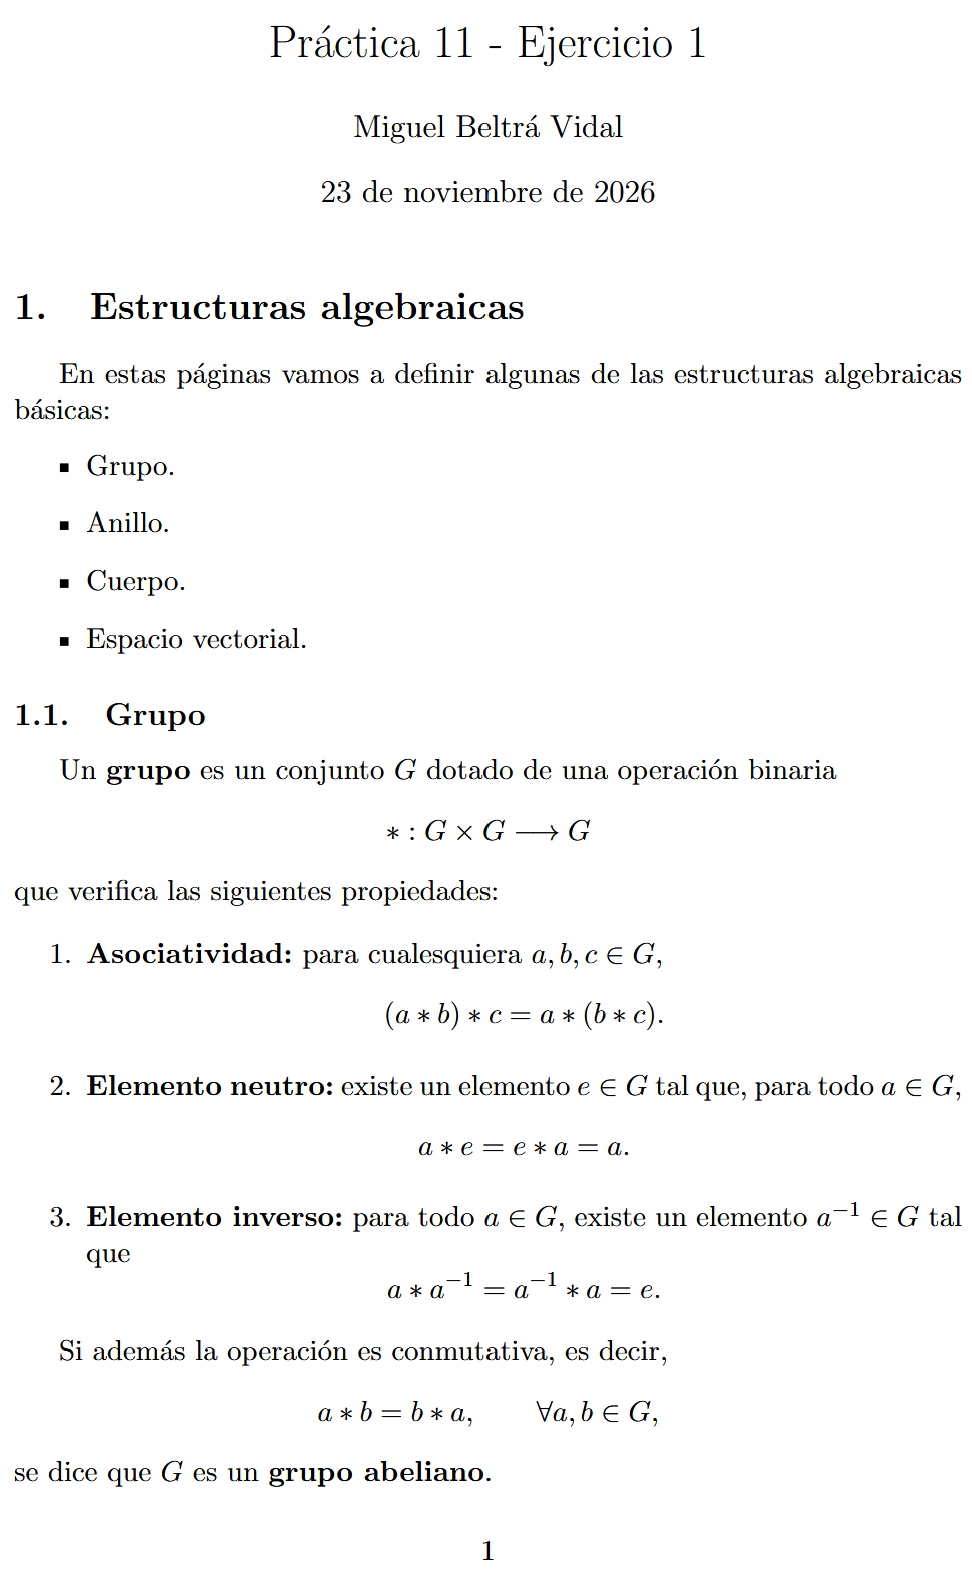
\includegraphics[width=0.85\linewidth]{images/exercise_1_1.png}
\end{center}
\end{paginarecuadrada}
\vfill

\newpage

\vfill
\begin{paginarecuadrada}
\begin{center}
	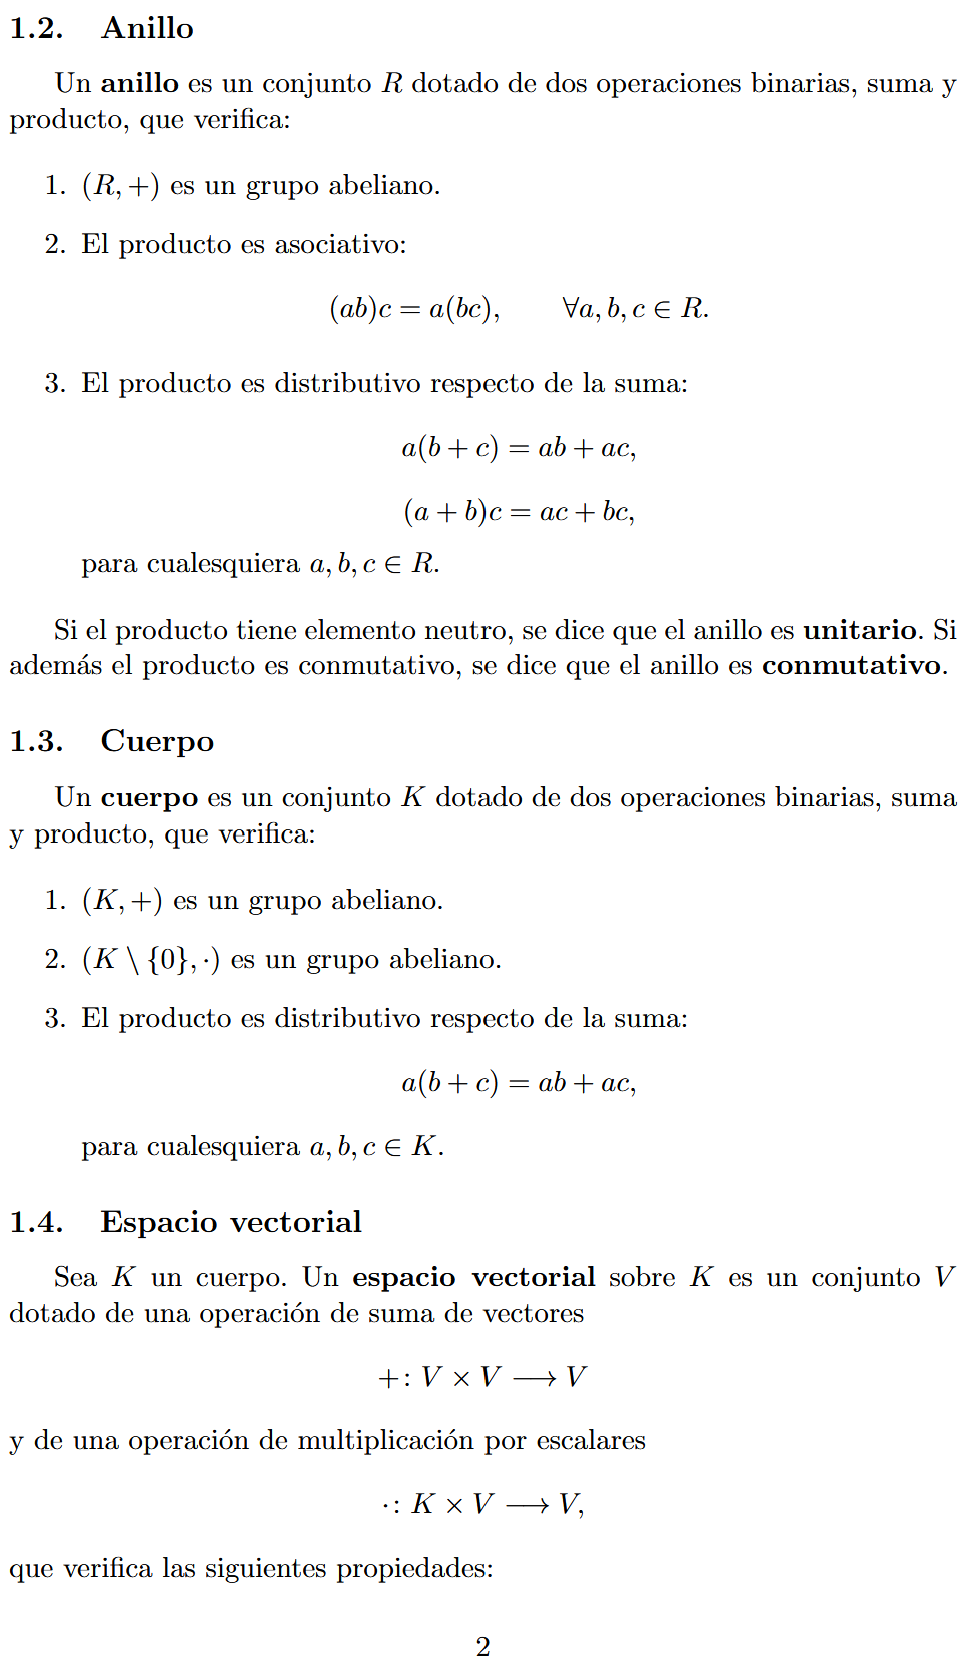
\includegraphics[width=0.85\linewidth]{images/exercise_1_2.png}
\end{center}
\end{paginarecuadrada}
\vfill

\newpage

\vfill
\begin{paginarecuadrada}
\begin{center}
	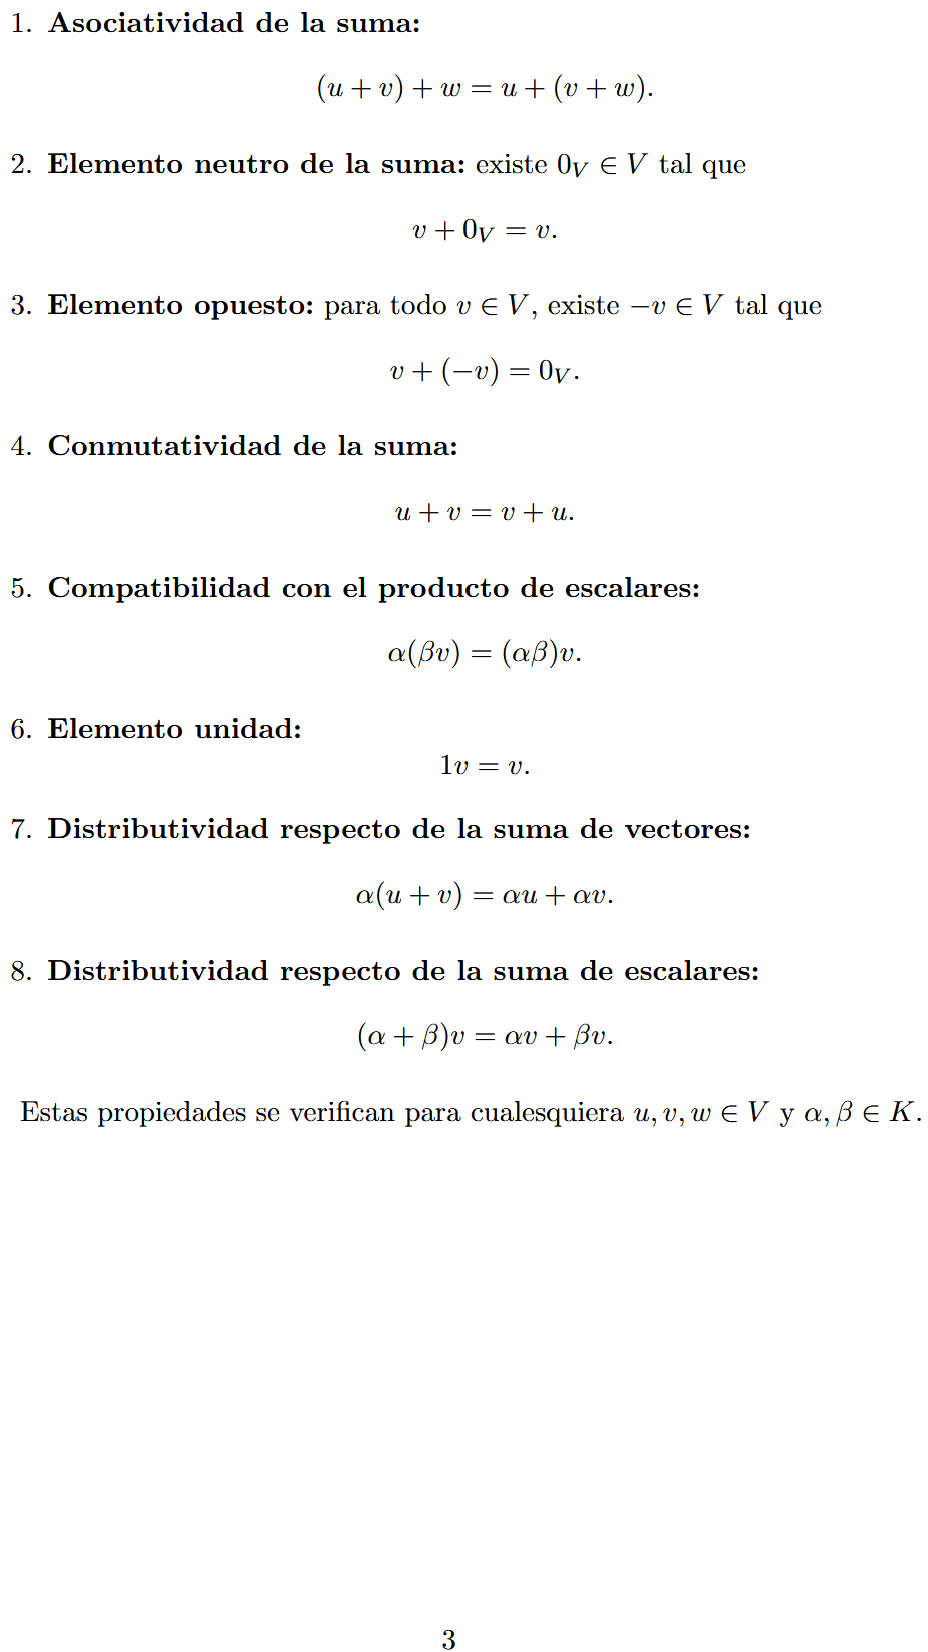
\includegraphics[width=0.85\linewidth]{images/exercise_1_3.png}
\end{center}
\end{paginarecuadrada}
\vfill
\end{exercise}




% =================================================
% 3. TABLAS Y MATRICES
% =================================================

\section{Tablas, arreglos y matrices}

\LaTeX\ permite construir estructuras tabulares tanto en modo texto como en modo matemático.

\subsection{Entorno \texttt{tabular}}

El entorno \verb|tabular| permite crear tablas. Su estructura general es:

\begin{center}
    \verb|\begin{tabular}{columnas}|
\end{center}

\noindent donde la especificación de las columnas indica cómo se alineará el contenido de cada una. Las opciones más habituales son:
\begin{itemize}
    \item \verb|l|: alinea el contenido a la izquierda.
    \item \verb|c|: centra el contenido.
    \item \verb|r|: alinea el contenido a la derecha.
    \item \texttt{|}: introduce una línea vertical para separar las columnas.
\end{itemize}

\noindent Para separar columnas se utiliza el carácter \verb|&| y para terminar una fila se utiliza \verb|\\|. El comando \verb|\hline| permite dibujar una línea horizontal.

\medskip

Por ejemplo, el siguiente código:

\begin{lstlisting}
\begin{center}
    \begin{tabular}{|l|c|r|}
        \hline
        Nombre & Edad & Nota \\ \hline
        Ana & 20 & 8.5 \\
        Luis & 21 & 7.2 \\
        Marta & 19 & 9.1 \\ \hline
    \end{tabular}
\end{center}
\end{lstlisting}

\noindent genera la siguiente tabla:

\begin{paginarecuadrada}
\begin{center}
    \begin{tabular}{|l|c|r|}
        \hline
        Nombre & Edad & Nota \\ \hline
        Ana & 20 & 8.5 \\
        Luis & 21 & 7.2 \\
        Marta & 19 & 9.1 \\ \hline
    \end{tabular}
\end{center}
\end{paginarecuadrada}

\medskip

%\noindent Podemos modificar la alineación de cada columna
%de manera independiente. Por ejemplo:
%
%\begin{lstlisting}
%\begin{center}
%    \begin{tabular}{|c|c|c|}
%        \hline
%        $x$ & $x^2$ & $x^3$ \\ \hline
%        1 & 1 & 1 \\
%        2 & 4 & 8 \\
%        3 & 9 & 27 \\ \hline
%    \end{tabular}
%\end{center}
%\end{lstlisting}
%
%\noindent genera la siguiente tabla:
%
%\begin{center}
%    \begin{tabular}{|c|c|c|}
%        \hline
%        $x$ & $x^2$ & $x^3$ \\ \hline
%        1 & 1 & 1 \\
%        2 & 4 & 8 \\
%        3 & 9 & 27 \\ \hline
%    \end{tabular}
%\end{center}

\subsection{Entorno \texttt{array}}

El entorno \verb|array| permite construir estructuras tabulares en modo matemático. Su funcionamiento es similar al de \verb|tabular|, pero se utiliza para organizar expresiones matemáticas. La sintaxis general es:

\begin{center}
    \verb|\begin{array}{columnas}|
\end{center}

\noindent Por ejemplo:

\begin{lstlisting}
\[
    \begin{array}{ccc}
        1 & 2 & 3 \\
        4 & 5 & 6 \\
        7 & 8 & 9
    \end{array}
\]
\end{lstlisting}

\noindent genera la siguiente estructura:

\begin{paginarecuadrada}
\[
    \begin{array}{ccc}
        1 & 2 & 3 \\
        4 & 5 & 6 \\
        7 & 8 & 9
    \end{array}
\]
\end{paginarecuadrada}

\medskip

\noindent También podemos utilizar líneas verticales y horizontales para separar columnas y filas:

\begin{lstlisting}
\[
    \begin{array}{|c|c|c|}
        \hline
        1 & 2 & 3 \\
        \hline
        4 & 5 & 6 \\
        \hline
        7 & 8 & 9 \\
        \hline
    \end{array}
\]
\end{lstlisting}

\noindent genera la siguiente estructura:

\begin{paginarecuadrada}
\[
    \begin{array}{|c|c|c|}
        \hline
        1 & 2 & 3 \\
        \hline
        4 & 5 & 6 \\
        \hline
        7 & 8 & 9 \\
        \hline
    \end{array}
\]
\end{paginarecuadrada}

\medskip

\noindent El entorno \verb|array| también permite organizar expresiones matemáticas de forma similar a una tabla. Por ejemplo, podemos escribir un sistema de ecuaciones:

\begin{lstlisting}
\[
    \left\{
        \begin{array}{rcl}
            x+y &=& 3 \\
            2x-y &=& 0
        \end{array}
    \right.
\]
\end{lstlisting}

\noindent Aquí, \verb|\right.| quiere decir que no se utiliza ningún delimitador en la derecha para cerrar el delimitador \verb|\left\{| abierto al inicio. El resultado será:

\begin{paginarecuadrada}
\[
    \left\{
        \begin{array}{rcl}
            x+y &=& 3 \\
            2x-y &=& 0
        \end{array}
    \right.
\]
\end{paginarecuadrada}


\subsection{Entorno \texttt{matrix}}

El paquete \verb|amsmath| proporciona diferentes entornos para escribir matrices. Entre ellos se encuentra \verb|matrix|, que permite construir matrices sin delimitadores.

\begin{lstlisting}
\[
    \begin{matrix}
        1 & 2 \\
        3 & 4
    \end{matrix}
\]
\end{lstlisting}

\noindent El resultado será:

\begin{paginarecuadrada}
\[
    \begin{matrix}
        1 & 2 \\
        3 & 4
    \end{matrix}
\]
\end{paginarecuadrada}

\medskip

\noindent Existen otras variantes que incorporan delimitadores:

\begin{itemize}
    \item \verb|pmatrix|: utiliza paréntesis.
    \item \verb|bmatrix|: utiliza corchetes.
    \item \verb|Bmatrix|: utiliza llaves.
    \item \verb|vmatrix|: utiliza barras verticales.
    \item \verb|Vmatrix|: utiliza barras verticales dobles.
\end{itemize}

\noindent Por ejemplo, el siguiente código:

\begin{lstlisting}
\[
    A=
    \begin{pmatrix}
        1 & 2 \\
        3 & 4
    \end{pmatrix}
\]
\end{lstlisting}

\noindent genera la siguiente matriz:

\begin{paginarecuadrada}
\[
    A=
    \begin{pmatrix}
        1 & 2 \\
        3 & 4
    \end{pmatrix}
\]
\end{paginarecuadrada}

\medskip

\noindent Si cambiamos el entorno por \verb|bmatrix|:

\begin{lstlisting}
\[
    A=
    \begin{bmatrix}
        1 & 2 \\
        3 & 4
    \end{bmatrix}
\]
\end{lstlisting}

\noindent obtendremos:

\begin{paginarecuadrada}
\[
    A=
    \begin{bmatrix}
        1 & 2 \\
        3 & 4
    \end{bmatrix}
\]
\end{paginarecuadrada}

\noindent Y si utilizamos \verb|Bmatrix|:

\begin{paginarecuadrada}
\[
    A=
    \begin{Bmatrix}
        1 & 2 \\
        3 & 4
    \end{Bmatrix}
    \qquad 
    B=
    \begin{vmatrix}
        1 & 2 \\
        3 & 4
    \end{vmatrix}
    \qquad
    C=
    \begin{Vmatrix}
        1 & 2 \\
        3 & 4
    \end{Vmatrix}
\]
\end{paginarecuadrada}

\medskip

\noindent Las matrices también pueden utilizarse para representar sistemas lineales, transformaciones y otras estructuras matemáticas.


\newpage
\begin{exercise} Crea un fichero llamado \texttt{ej2.tex}. El contenido del fichero debe generar el siguiente documento de \LaTeX. En tu repositorio de \Git\ deberás llevar un seguimiento tanto del fichero \texttt{ej2.tex} como del documento \texttt{ej2.pdf} generado y subirlo a \GitHub.

\vfill
\begin{paginarecuadrada}
\begin{center}
	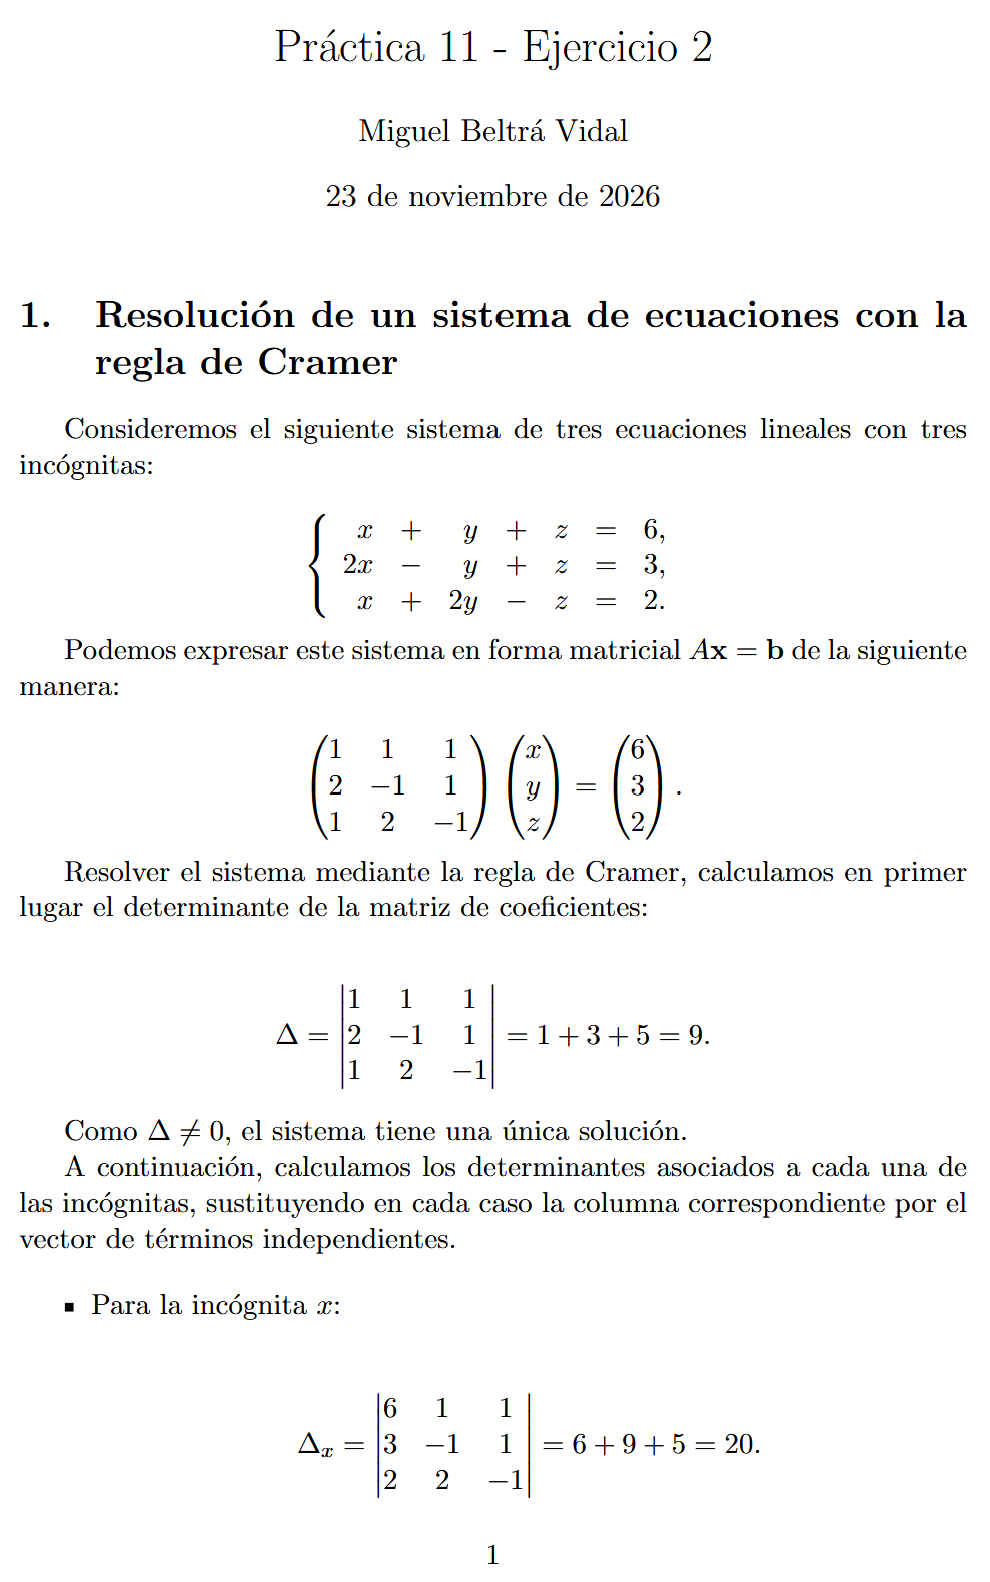
\includegraphics[width=0.85\linewidth]{images/exercise_2_1.png}
\end{center}
\end{paginarecuadrada}
\vfill


\begin{paginarecuadrada}
\begin{center}
	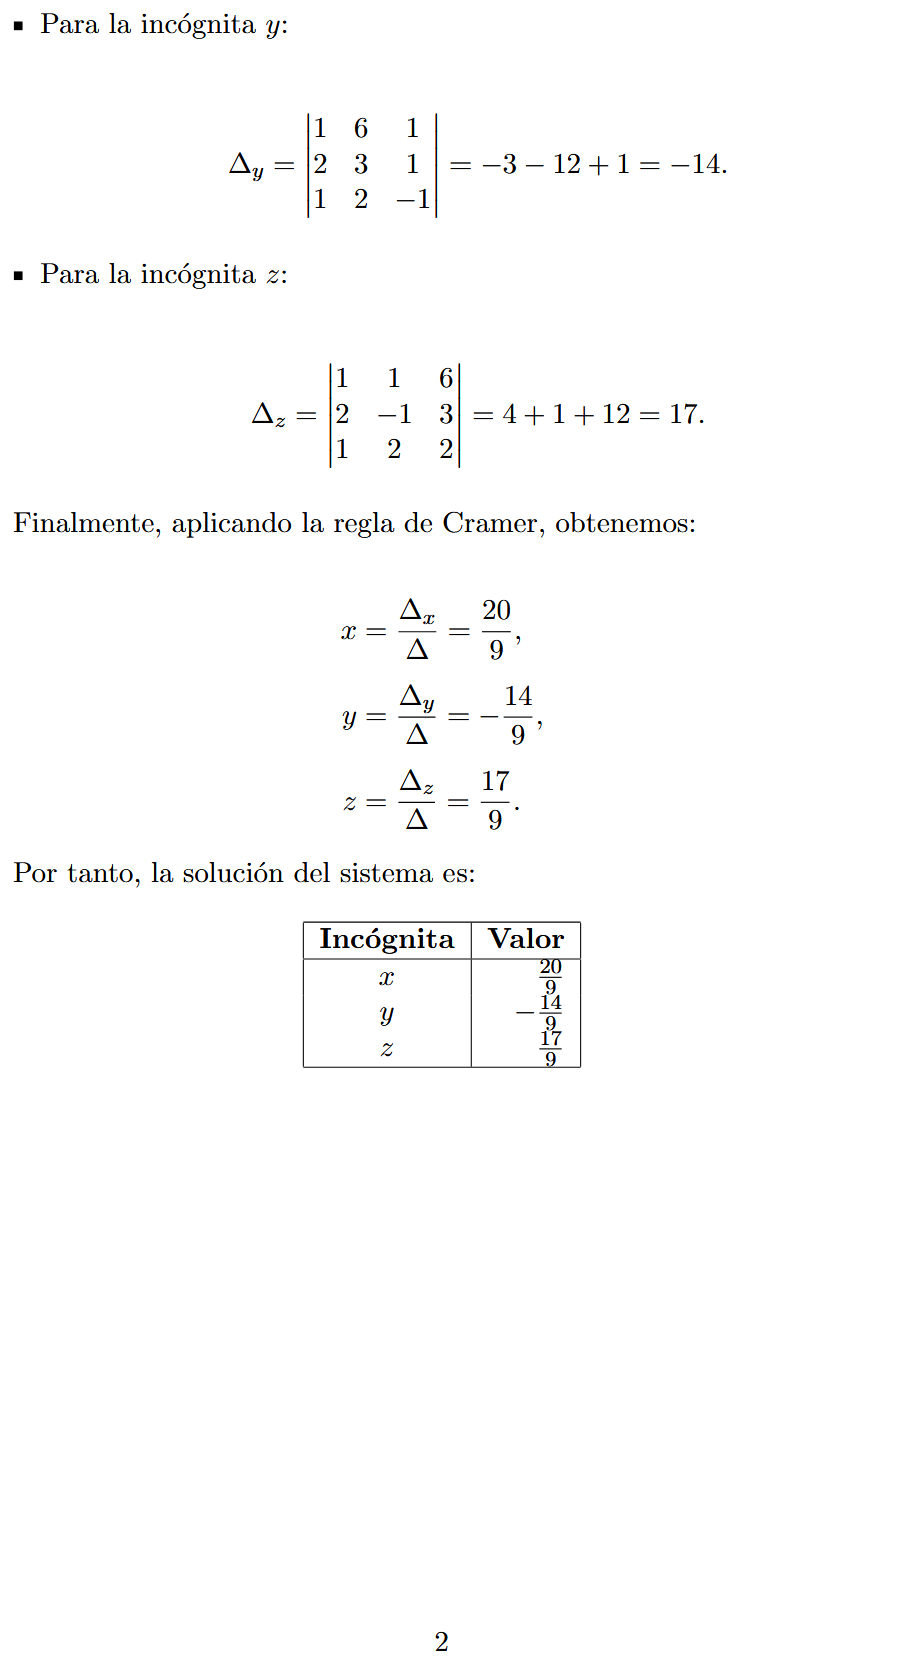
\includegraphics[width=0.85\linewidth]{images/exercise_2_2.png}
\end{center}
\end{paginarecuadrada}
\end{exercise}

\newpage



% =================================================
% 4. ALINEACIÓN DE ECUACIONES
% =================================================

\section{Alineación de ecuaciones}

El entorno \verb|align*| del paquete \verb|amsmath| permite escribir varias expresiones matemáticas alineadas entre sí. Al igual que con los entornos \texttt{tabular}, \texttt{array} y \texttt{matrix}, las posiciones de alineación se indican mediante el carácter \verb|&| y cada línea se termina con \verb|\\|.

%\subsection{Entorno \texttt{align}}
%
%Por ejemplo, el código siguiente:
%
%\begin{lstlisting}
%\begin{align}
%    x+y &= 3 \\
%    2x-y &= 0
%\end{align}
%\end{lstlisting}
%
%\noindent genera las ecuaciones siguientes:
%
%\begin{align}
%    x+y &= 3 \\
%    2x-y &= 0
%\end{align}
%
%\medskip
%
%\noindent En este caso, las ecuaciones se alinean en
%el signo de igualdad. El carácter \verb|&| indica
%la posición en la que debe realizarse la alineación.
%
%\medskip
%
%\noindent Podemos escribir varias líneas de cálculos
%matemáticos. Por ejemplo:
%
%\begin{lstlisting}
%\begin{align}
%    (x+1)^2 &= x^2+2x+1 \\
%             &= x^2+x+x+1 \\
%             &= x(x+2)+1
%\end{align}
%\end{lstlisting}
%
%\noindent El resultado será:
%
%\begin{align}
%    (x+1)^2 &= x^2+2x+1 \\
%             &= x^2+x+x+1 \\
%             &= x(x+2)+1
%\end{align}
%
%\medskip
%
%\noindent También podemos alinear expresiones en
%varios puntos:
%
%\begin{lstlisting}
%\begin{align}
%    f(x) &= x^2+2x+1 \\
%         &= (x+1)^2 \\
%    g(x) &= x^3-1 \\
%         &= (x-1)(x^2+x+1)
%\end{align}
%\end{lstlisting}
%
%\noindent El resultado será:
%
%\begin{align}
%    f(x) &= x^2+2x+1 \\
%         &= (x+1)^2 \\
%    g(x) &= x^3-1 \\
%         &= (x-1)(x^2+x+1)
%\end{align}

\subsection{Entorno \texttt{align*}}

El entorno \verb|align| numera automáticamente las ecuaciones. Si queremos evitar la numeración, podemos utilizar su versión con asterisco:
\verb|align*|.

\begin{lstlisting}
\begin{align*}
    x+y  & = 3 \\
    2x-y & = 0
\end{align*}
\end{lstlisting}

\noindent El resultado será:

\begin{paginarecuadrada}
\begin{align*}
    x+y  & = 3 \\
    2x-y & = 0
\end{align*}
\end{paginarecuadrada}

\medskip

\noindent De esta manera, podemos escribir expresiones alineadas sin que aparezcan números junto a ellas. También podemos alinear varios conjuntos de ecuaciones:

\begin{lstlisting}
\begin{align*}
    x+y  & = 3 &  x-y & = 4 & x+y & = 1 \\
    2x-y & = 0 & 3x-y & = 6 &  2y & = 4
\end{align*}
\end{lstlisting}

\noindent El resultado será:

\begin{paginarecuadrada}
\begin{align*}
    x+y  & = 3 &  x-y & = 4 & x+y & = 1 \\
    2x-y & = 0 & 3x-y & = 6 &  2y & = 4
\end{align*}
\end{paginarecuadrada}

 
\subsection{El entorno \texttt{cases}}

El entorno \texttt{cases}, proporcionado por el paquete \texttt{amsmath}, permite escribir funciones definidas a trozos y otras expresiones en las que se presentan varios casos agrupados bajo una llave a la izquierda. Cada fila del entorno representa un caso distinto. Se utiliza el símbolo \texttt{\&} para separar la expresión del valor o condición que la acompaña, y \texttt{\textbackslash\textbackslash} para pasar a la siguiente fila. 

\medskip

Por ejemplo, para representar una función definida a trozos, podemos escribir:

\begin{lstlisting}
\[
	f(x)=
	\begin{cases}
		x^2, & \text{si } x \geq 0, \\
		-x,  & \text{si } x < 0.
	\end{cases}
\]
\end{lstlisting}

\noindent El resultado será:

\begin{paginarecuadrada}
\[
f(x)=
\begin{cases}
x^2, & \text{si } x \geq 0, \\
-x,  & \text{si } x < 0.
\end{cases}
\]
\end{paginarecuadrada}


Obsérvese que el entorno \texttt{cases} coloca automáticamente una llave a la izquierda, alinea las expresiones a partir del símbolo \texttt{\&} y ajusta el espaciado entre las filas. Asimismo, el texto que aparece dentro de las expresiones matemáticas debe introducirse mediante \texttt{\textbackslash text\{\}}, para que se muestre con tipografía normal.

\medskip

También podemos utilizar el entorno \texttt{cases} para expresar otras situaciones, como el valor absoluto de un número:

\begin{lstlisting}
\[
	\lvert x \rvert =
	\begin{cases}
		x,  & \text{si } x \geq 0, \\
		-x, & \text{si } x < 0.
	\end{cases}
\]
\end{lstlisting}

\noindent El resultado será:

\begin{paginarecuadrada}
\[
	\lvert x \rvert =
	\begin{cases}
		x,  & \text{si } x \geq 0,\\
		-x, & \text{si } x < 0.
	\end{cases}
\]
\end{paginarecuadrada}



\newpage
\begin{exercise} Crea un fichero llamado \texttt{ej3.tex}. El contenido del fichero debe generar el siguiente documento de \LaTeX. Para poner las flechas de vectores, deberás usar el comando \verb|\vec{...}|. Por ejemplo, \verb|\vec{v}| produce $\vec{v}$. En tu repositorio de \Git\ deberás llevar un seguimiento tanto del fichero \texttt{ej3.tex} como del documento \texttt{ej3.pdf} generado y subirlo a \GitHub.

\vfill
\begin{paginarecuadrada}
\begin{center}
	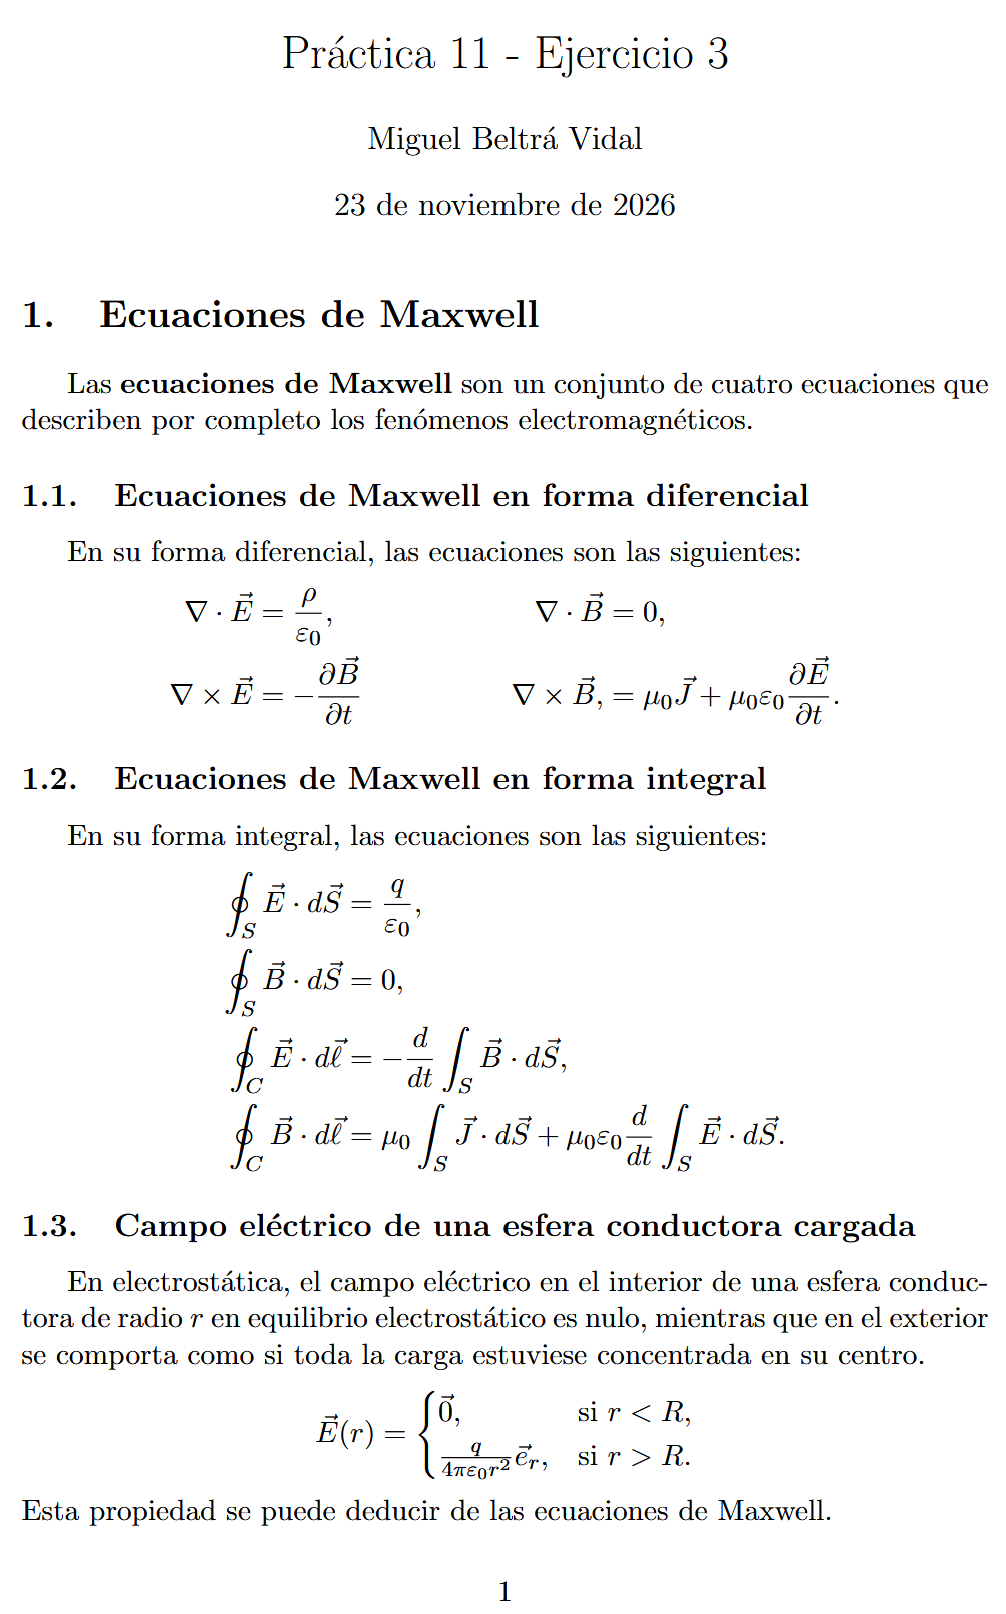
\includegraphics[width=0.85\linewidth]{images/exercise_3.png}
\end{center}
\end{paginarecuadrada}
\vfill
\end{exercise}

\newpage

% =================================================
% 5. ENTORNOS MATEMÁTICOS
% =================================================

\section{Entornos matemáticos}

En documentos matemáticos es habitual utilizar entornos específicos para presentar definiciones, teoremas, proposiciones, lemas, corolarios y demostraciones. El paquete \verb|amsthm| proporciona herramientas para crear este tipo de entornos y personalizar su formato.

\subsection{Entornos predefinidos}

El paquete \verb|amsthm| proporciona el entorno \verb|proof| para escribir demostraciones. Por ejemplo:

\begin{lstlisting}
\begin{proof}
    La demostracion se desarrolla a continuacion.
\end{proof}
\end{lstlisting}

\noindent El resultado será:

\begin{paginarecuadrada}
\begin{proof}[Proof]
    La demostración se desarrolla a continuación.
\end{proof}
\end{paginarecuadrada}

\medskip

\noindent El entorno \verb|proof| incluye automáticamente el encabezado ``\emph{Proof}''. Si tenemos el documento configurado en otro idioma entonces se incluirá este encabezado traducido. Por ejemplo, si hemos cargado \verb|\usepackage[spanish]{babel}|, entonces el encabezado será ``\emph{Demostración}'':

\begin{lstlisting}
\begin{proof}
    La demostracion se desarrolla a continuacion.
\end{proof}
\end{lstlisting}

\noindent El resultado será:

\begin{paginarecuadrada}
\begin{proof}
    La demostración se desarrolla a continuación.
\end{proof}
\end{paginarecuadrada}

\noindent Podemos modificar el encabezado de la demostración mediante un argumento opcional:

\begin{lstlisting}
\begin{proof}[Esbozo de la demostracion]
    Las ideas clave de la demostracion son las siguientes:
\end{proof}
\end{lstlisting}

\noindent El resultado será:

\begin{paginarecuadrada}
\begin{proof}[Esbozo de la demostracion]
    Las ideas clave de la demostracion son las siguientes:
\end{proof}
\end{paginarecuadrada}

\subsection{Definición de entornos propios}

Para crear nuestros propios entornos matemáticos utilizamos el comando \verb|\newtheorem| en el preámbulo del documento. La sintaxis general es:

\begin{center}
    \verb|\newtheorem{nombre}{titulo}|
\end{center}

\noindent Por ejemplo, podemos definir un entorno para escribir teoremas:

\begin{lstlisting}
\newtheorem{teorema}{Teorema}
\end{lstlisting}

\noindent Esta definición debe incluirse en el preámbulo, antes de \verb|\begin{document}|. Una vez definido el entorno, podemos utilizarlo en el documento:

\begin{lstlisting}
\begin{teorema}
    Todo numero natural es positivo o cero.
\end{teorema}
\end{lstlisting}

\noindent El resultado será:

\begin{paginarecuadrada}
\begin{teorema}
    Todo número natural es positivo o cero.
\end{teorema}
\end{paginarecuadrada}

\medskip

\noindent La numeración de los teoremas se genera automáticamente. Si definimos varios entornos utilizando el mismo contador, podemos conseguir que todos compartan una numeración común.

\medskip

\noindent Por ejemplo, en el preámbulo:

\begin{lstlisting}
\newtheorem{teorema}{Teorema}
\newtheorem{proposicion}[teorema]{Proposicion}
\newtheorem{corolario}[teorema]{Corolario}
\end{lstlisting}

\noindent En este caso, los entornos \verb|teorema|, \verb|proposicion| y \verb|corolario| comparten la numeración. Si utilizamos los tres entornos:

\begin{lstlisting}
\begin{teorema}
    Enunciado de un teorema.
\end{teorema}

\begin{proposicion}
    Enunciado de una proposicion.
\end{proposicion}

\begin{corolario}
    Enunciado de un corolario.
\end{corolario}
\end{lstlisting}

\noindent la numeración será consecutiva entre los tres tipos de enunciados.

\begin{paginarecuadrada}
\begin{teorema}
    Enunciado de un teorema.
\end{teorema}

\begin{proposicion}
    Enunciado de una proposicion.
\end{proposicion}

\begin{corolario}
    Enunciado de un corolario.
\end{corolario}
\end{paginarecuadrada}


\subsection{Estilos de los entornos}

El paquete \verb|amsthm| permite modificar el estilo de los entornos definidos mediante el comando \verb|\theoremstyle|. Los principales estilos son:

\begin{itemize}
    \item \verb|plain|: el texto aparece en cursiva. Es el estilo habitual para teoremas, proposiciones y corolarios.
    \item \verb|definition|: el texto aparece en letra normal. Es adecuado para definiciones y ejemplos.
    \item \verb|remark|: el texto aparece en letra normal y el encabezado tiene un estilo diferente. Es habitual utilizarlo para observaciones.
\end{itemize}

\noindent Por ejemplo, podemos definir diferentes entornos en el preámbulo:

\begin{lstlisting}
\theoremstyle{plain}
\newtheorem{teorema}{Teorema}
\newtheorem{lema}[teorema]{Lema}

\theoremstyle{definition}
\newtheorem{definicion}{Definicion}
\newtheorem{ejemplo}{Ejemplo}

\theoremstyle{remark}
\newtheorem{observacion}{Observacion}
\end{lstlisting}

\medskip

\noindent A continuación, podemos utilizarlos en
el documento:

\begin{lstlisting}
\begin{definicion}
    Un numero primo es un numero natural mayor que uno que tiene 
    exactamente dos divisores positivos.
\end{definicion}

\begin{teorema}
    Existen infinitos numeros primos.
\end{teorema}

\begin{observacion}
    El numero 2 es el unico numero primo par.
\end{observacion}
\end{lstlisting}

\noindent El resultado será:

\begin{paginarecuadrada}
\begin{definicion}
    Un número primo es un número natural mayor que uno que tiene exactamente dos divisores
    positivos.
\end{definicion}

\begin{teorema}
    Existen infinitos números primos.
\end{teorema}

\begin{observacion}
    El número 2 es el único número primo par.
\end{observacion}
\end{paginarecuadrada}

\medskip

\noindent Podemos incluir un argumento opcional para
añadir información al título del entorno. Por ejemplo:

\begin{lstlisting}
\begin{teorema}[Teorema fundamental]
    Enunciado del teorema.
\end{teorema}
\end{lstlisting}

\noindent El título aparecerá junto al nombre y al
número del teorema.

\begin{paginarecuadrada}
\begin{teorema}[Teorema fundamental]
    Enunciado del teorema.
\end{teorema}
\end{paginarecuadrada}


\subsection{Numeración por secciones}

También podemos hacer que la numeración de los entornos matemáticos dependa de las secciones
del documento. Para ello, utilizamos un argumento adicional en el comando \verb|\newtheorem|:

\begin{lstlisting}
\newtheorem{teorema}{Teorema}[section]
\end{lstlisting}

\noindent En este caso, los teoremas se numerarán teniendo en cuenta la sección en la que aparecen. Por ejemplo, el primer teorema de la sección 2 será el Teorema 2.1.

\medskip

\noindent Si queremos que otros entornos compartan
esta numeración, podemos utilizar:

\begin{lstlisting}
\newtheorem{teorema}{Teorema}[section]
\newtheorem{proposicion}[teorema]{Proposicion}
\newtheorem{corolario}[teorema]{Corolario}
\end{lstlisting}

\noindent De esta forma, teoremas, proposiciones y corolarios compartirán el mismo contador, que se reiniciará al comenzar una nueva sección.




\newpage
\begin{exercise} Crea un fichero llamado \texttt{ej4.tex}. El contenido del fichero debe generar el siguiente documento de \LaTeX. En tu repositorio de \Git\ deberás llevar un seguimiento tanto del fichero \texttt{ej4.tex} como del documento \texttt{ej4.pdf} generado y subirlo a \GitHub.

\vfill
\begin{paginarecuadrada}
\begin{center}
	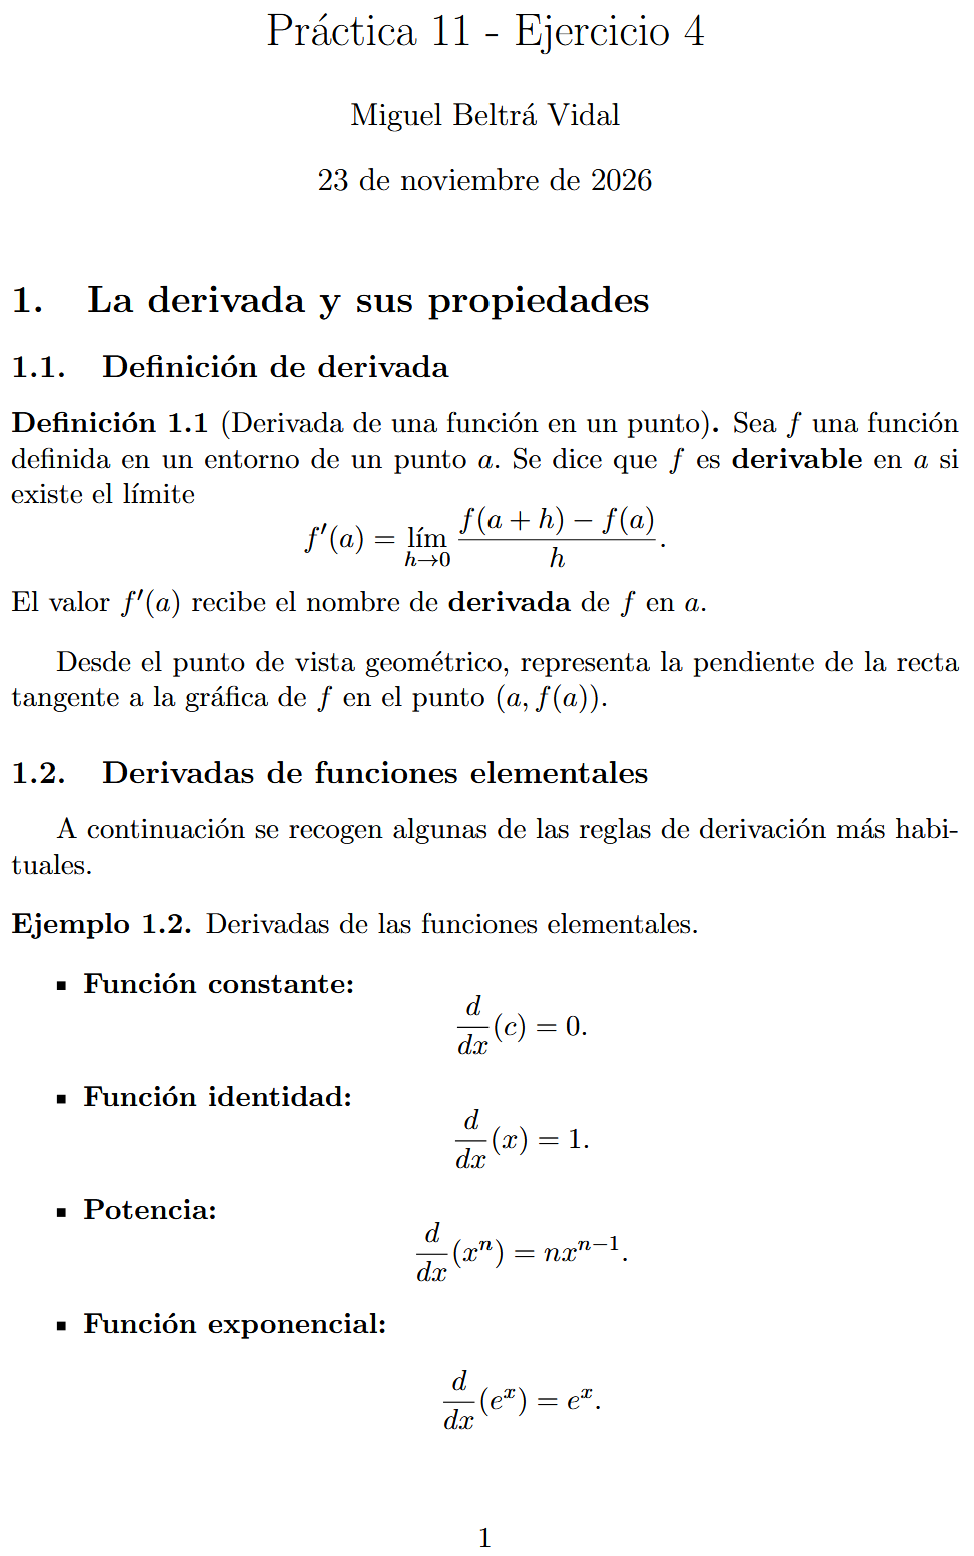
\includegraphics[width=0.85\linewidth]{images/exercise_4_1.png}
\end{center}
\end{paginarecuadrada}
\vfill

\newpage

\vfill
\begin{paginarecuadrada}
\begin{center}
	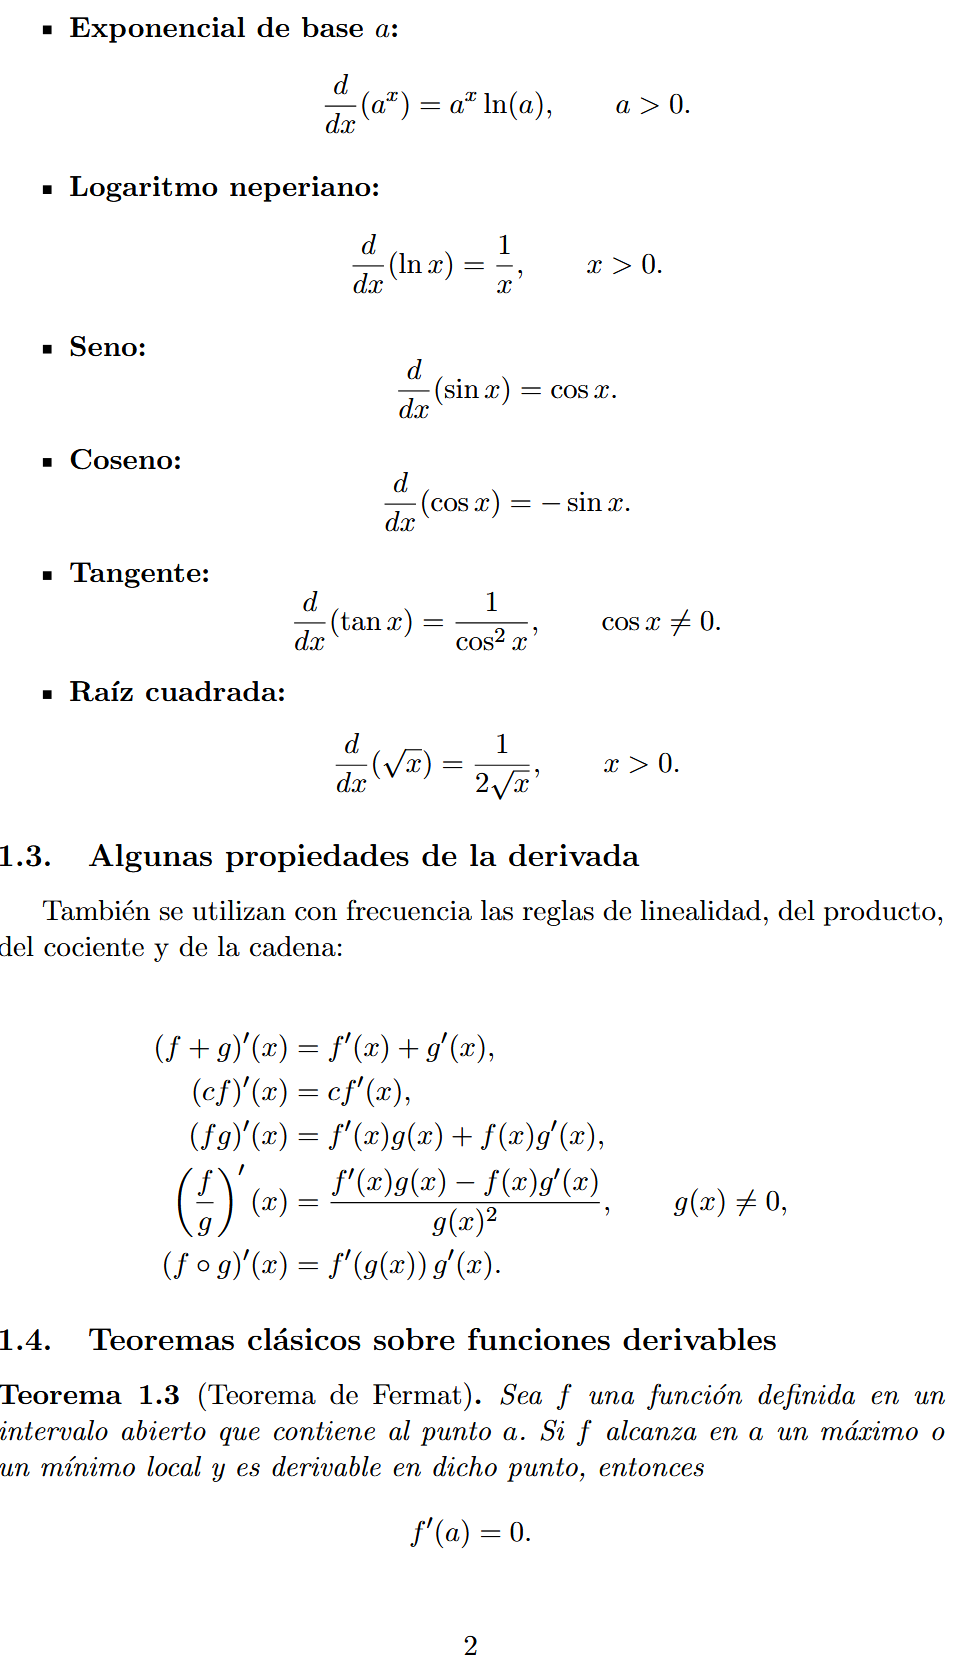
\includegraphics[width=0.85\linewidth]{images/exercise_4_2.png}
\end{center}
\end{paginarecuadrada}
\vfill

\newpage

\vfill
\begin{paginarecuadrada}1
\begin{center}
	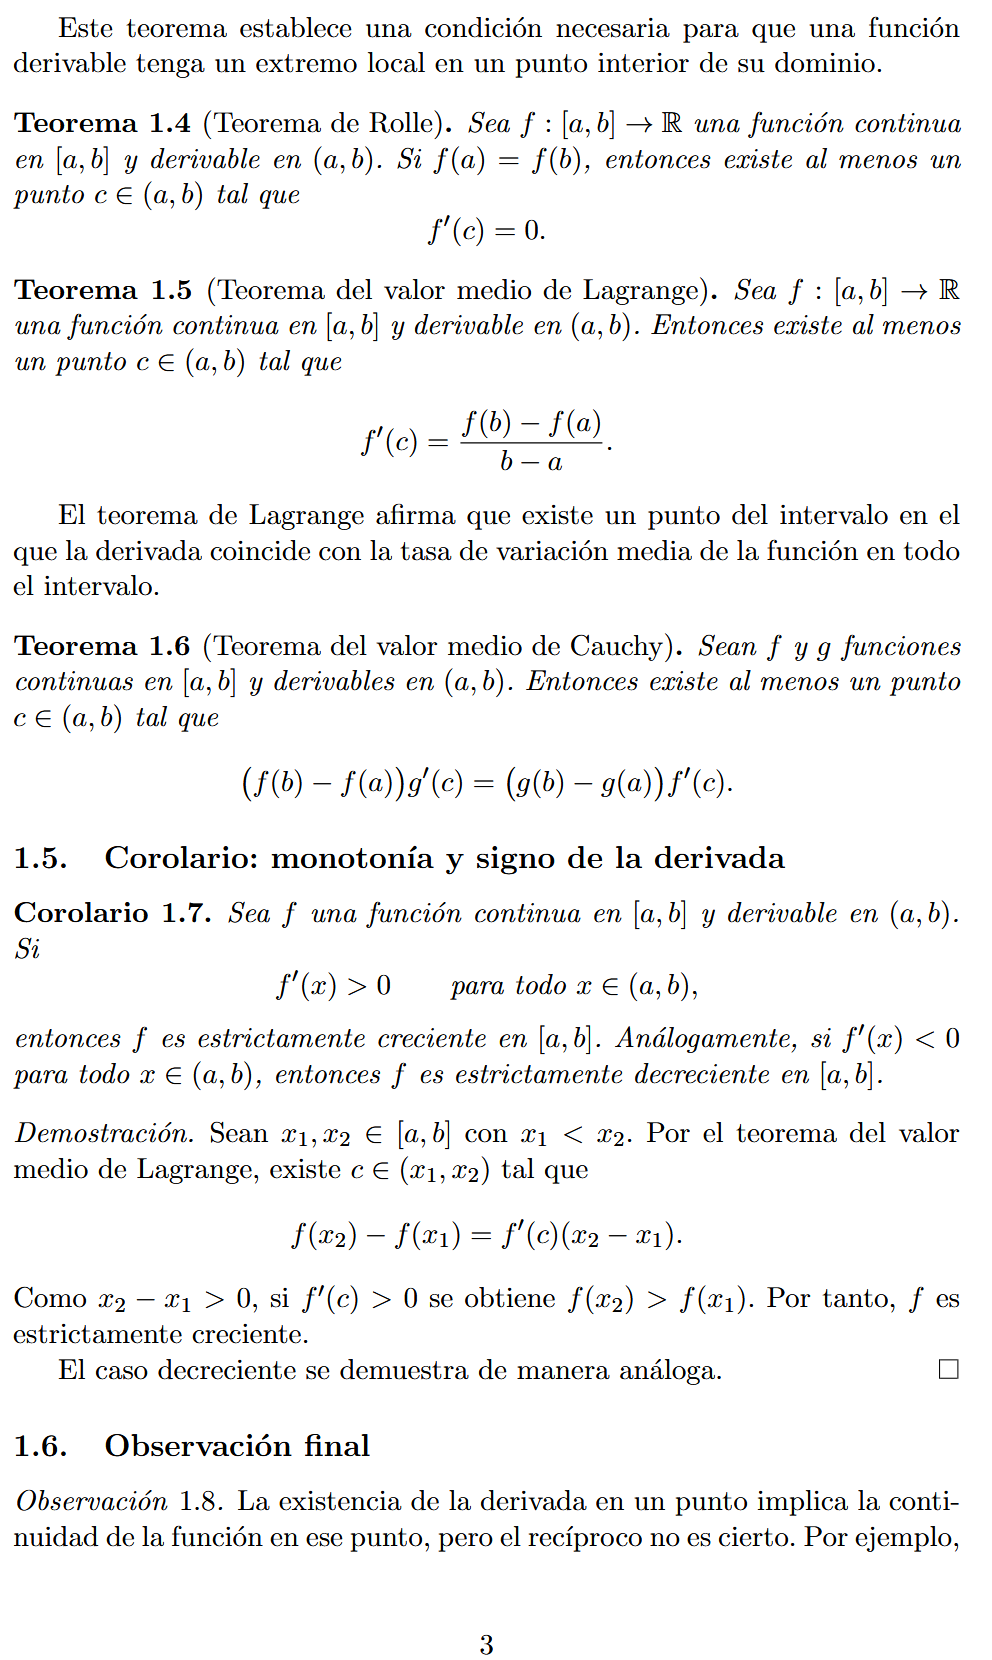
\includegraphics[width=0.85\linewidth]{images/exercise_4_3.png}
\end{center}
\end{paginarecuadrada}
\vfill

\newpage

\vfill
\begin{paginarecuadrada}
\begin{center}
	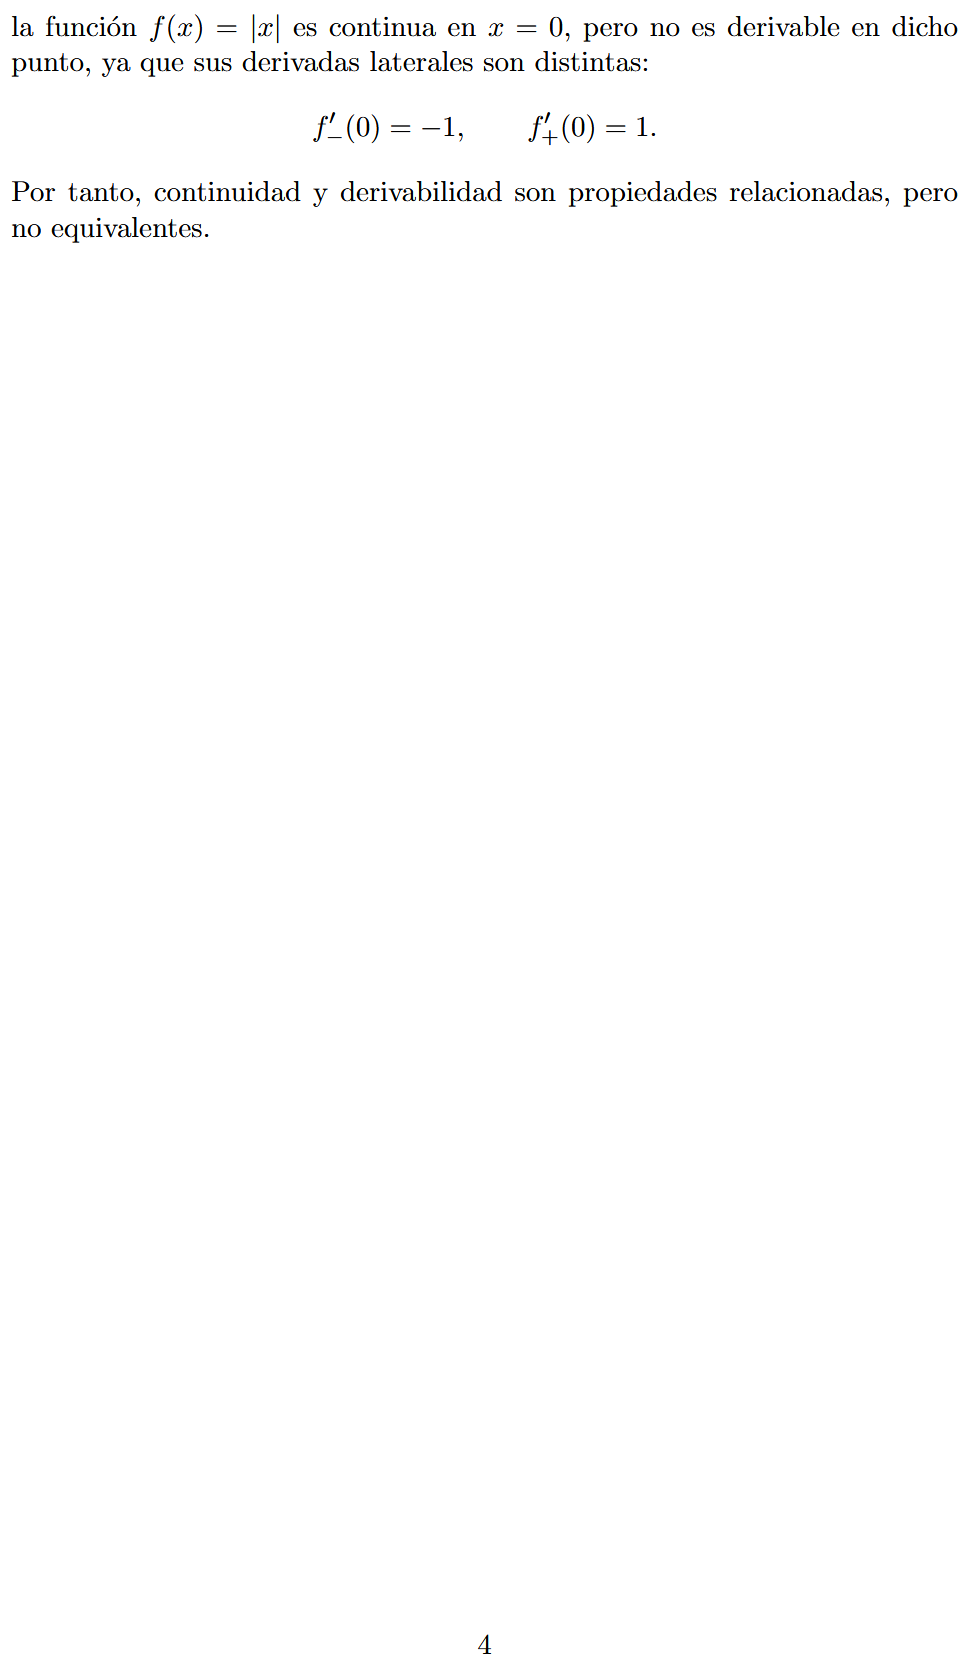
\includegraphics[width=0.85\linewidth]{images/exercise_4_4.png}
\end{center}
\end{paginarecuadrada}
\vfill
\end{exercise}




% =================================================
% 6. DOCUMENTACIÓN
% =================================================

\section{Documentación del código}

El código debe estar correctamente organizado y comentado. El objetivo no es únicamente conseguir que el PDF se genere correctamente, sino escribir código fácil de leer y modificar.


\begin{exercise} Crea un fichero \texttt{README.md} para documentar esta práctica. El aspecto deberá ser similar al de las prácticas anteriores.
\end{exercise}

\section{Entrega}

Sube los ficheros correspondientes a la práctica a tu \GitHub\ en la fecha acordada con el profesor. Para esta práctica:
\begin{enumerate}
    \item Guarda los ficheros \texttt{.tex} en la carpeta de la práctica correspondiente.
    \item Utiliza nombres de fichero claros y consistentes.
    \item Comprueba que el documento \texttt{.pdf} se genera correctamente.
\end{enumerate}
Después de esta práctica, la estructura de directorios de tu repositorio se debería parecer a la siguiente:

\begin{center}
\begin{minipage}{0.75\linewidth}
\dirtree{%
    .1 \faIcon[regular]{folder-open}\ practicas/.
	    .2 \faIcon[regular]{folder-open}\ .git/.
        .2 \faIcon[regular]{folder-open}\ assets/.
            .3 \faIcon[regular]{folder-open}\ images/.
        .2 \faIcon[regular]{folder-open}\ Git/.
        .2 \faIcon[regular]{folder-open}\ R/.
        .2 \faIcon[regular]{folder-open}\ LaTeX/.
        		.3 \faIcon[regular]{folder-open}\ practica\_10/.
        		.3 \faIcon[regular]{folder-open}\ practica\_11/.
		        .4 \faIcon[regular]{file-alt}\ ej1.tex.
		        .4 \faIcon[regular]{file-pdf}\ ej1.pdf.
		        .4 \faIcon[regular]{file-alt}\ ej2.tex.
		        .4 \faIcon[regular]{file-pdf}\ ej2.pdf.
		        .4 \faIcon[regular]{file-alt}\ ej3.tex.
		        .4 \faIcon[regular]{file-pdf}\ ej3.pdf.
		        .4 \faIcon[regular]{file-alt}\ README.md.
        .2 \faIcon[regular]{file-alt}\ .gitignore.
        .2 \faIcon[regular]{file-alt}\ README.md.
}
\end{minipage}
\end{center}


\end{document}